\documentclass[12pt,a4paper,twocolumn]{article}
\usepackage[utf8]{inputenc}
\usepackage[T1]{fontenc}
\usepackage{polski}
\usepackage[polish]{babel}
\usepackage{geometry}
\geometry{margin=2.5cm}
\usepackage{graphicx}
\usepackage{tabularx}
\usepackage{booktabs} 
\usepackage{hyperref}
\usepackage{bookmark}
\usepackage{enumitem}
\usepackage{titlesec}

\title{
    \begin{center}
    
\includegraphics[width=\textwidth]{fig/logo.png}
    \vspace{0.25cm}
    \end{center}
    \textbf{\huge Struktury danych} \\
    \vspace{0.5cm}
    \textit{Analiza porównawcza wydajności list wiązanych i tablic dynamicznych w języku C++}
}
\author{Piotr Frąc}
\date{Marzec 2026}


\begin{document}
\maketitle

\section{Wprowadzenie}
Projekt skupia się na analizie porównawczej dwóch fundamentalnych struktur liniowych:
\textit{linked list} i \textit{dynamic array} \\ 
Celem pracy jest implementacja obu struktur w języku C++ 
oraz przeprowadzenie testów wydajnościowych dla podstawowych operacji, takich jak:

\begin{itemize}[nosep]
\item dodawanie i usuwanie elementów (na początku, na końcu oraz na zadanym indeksie),
\item wyszukiwanie elementów o określonej wartości,
\item dostęp do elementu poprzez indeks. 
\end{itemize}

Badanie ma na celu wykazanie różnic w złożoności obliczeniowej oraz praktycznym czasie wykonania, 
wynikających ze specyfiki alokacji pamięci
Pełny kod źródłowy projektu wraz z historią zmian dostępny jest w repozytorium pod adresem: 
\url{https://github.com/Elrior-programmer/Struktury-Danych/tree/main/P1%20-%20Lista_wizana} 
\subsection{Zaimplementowane \\ struktury danych}
Wszystkie struktury danych zostały wykonane zgodnie z wykładami i prezentacjami dr inż. Radosława Rudego, które są dostępne pod linkiem: 
\url{https://kam.pwr.edu.pl/jaroslaw-rudy/#tab-struktury-danych-wyklad}
\subsubsection*{Lista wiązana}
Zaimplementowana \textbf{lista} jest przykładem \textit{Listy jednokierunkowej liniowej (Singly Linked List)}, 
\begin{center}
    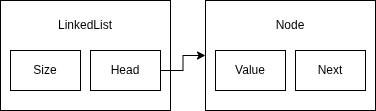
\includegraphics[width=\linewidth]{fig/LinkedList.png}
\end{center}
która charakteryzuje sie:
\begin{itemize}[nosep]
\item \textbf{Jednokierunkowość:} Każdy węzeł (\textit{node})
 przechowuje wskaźnik wyłącznie do swojego następcy. 
 Oznacza to, że przeglądanie struktury możliwe jest tylko od głowy (\textit{head})
w stronę końca listy.

\item \textbf{Liniowość (brak cyliczności):} 
Struktura posiada wyraźnie zdefiniowany początek oraz koniec.
Ostatni element przechowuje wartość pustą (\texttt{nullptr}),
co stanowi jednoznacznie zakończenie sekwencji danych.
\end{itemize}
sprawdzam ile liniej do nowej strony \\
sprawdzam ile liniej do nowej strony \\
\end{document}